%!TEX root = ../../Heun_Dale_Haney_A_dynamic_approach_to_input_output_modeling.tex
%%%%%%%%%%%%%%%%%%%%% chapter.tex %%%%%%%%%%%%%%%%%%%%%%%%%%%%%%%%%
%
% sample chapter
%
% Use this file as a template for your own input.
%
%%%%%%%%%%%%%%%%%%%%%%%% Springer-Verlag %%%%%%%%%%%%%%%%%%%%%%%%%%
%\motto{Use the template \emph{chapter.tex} to style the various elements of your chapter content.}
\motto{Need a motto.~\emph{\cite[p.~26]{Berry1998}}

\hfill---\emph{Wendell Berry}}


%%%%%%%%%%%%%%%%%%%%%%%%%%%%%%%%%%
%%%%%%%%%% Introduction %%%%%%%%%%
%%%%%%%%%%%%%%%%%%%%%%%%%%%%%%%%%%
\chapter{Introduction: The end of an era}
% Always give a unique label
\label{chap:intro}
% use \chaptermark{}
% to alter or adjust the chapter heading in the running head
\chaptermark{Introduction}
%%%%%%%%%%%%%%%%%%%%%%%%%%%%%%%%%%
%%%%%%%%%%%%%%%%%%%%%%%%%%%%%%%%%%
%%%%%%%%%%%%%%%%%%%%%%%%%%%%%%%%%%


%% \abstract{Each chapter should be preceded by an abstract (10--15 lines long) that summarizes the content. The abstract will appear \textit{online} at \url{www.SpringerLink.com} and be available with unrestricted access. This allows unregistered users to read the abstract as a teaser for the complete chapter. As a general rule the abstracts will not appear in the printed version of your book unless it is the style of your particular book or that of the series to which your book belongs.\newline\indent
%% Please use the 'starred' version of the new Springer \texttt{abstract} command for typesetting the text of the online abstracts (cf. source file of this chapter template \texttt{abstract}) and include them with the source files of your manuscript. Use the plain \texttt{abstract} command if the abstract is also to appear in the printed version of the book.}

%% Use the template \emph{chapter.tex} together with the Springer document class SVMono (monograph-type books) or SVMult (edited books) to style the various elements of your chapter content in the Springer layout.

\abstract*{**** Re-write the abstract. ****
In this chapter we give our motivation for writing this book. 
We outline some of the models and subsequent metaphors 
that have been used to describe the economy---clockwork, 
machine, engine---and suggest a new metaphor---the 
metabolism of an organism.
We give an overview of Leontief Input-Output methods
and their extension to include energy and material inputs
and waste flows out of the economy.
We then propose a new Input-Output analysis method,
fitting to the new metaphor of the metabolic economy;
a dynamic accounting framework that includes accumulation of stocks
within economic sectors.}




%%%%%%%%%% Growth has stalled %%%%%%%%%%
\section{[BRH] Economic growth  has stalled for mature economies}
\label{sec:growth_has_slowed}
%%%%%%%%

The world is entering a new economic era. There is widespread agreement that economic growth in mature economies is unlikely to reach the rates seen in the 20th century again.  The OECD data show that during the 20th century, average growth rates for the developed world ranged from 2 to 4\%. The long-term forecast from the OECD is that mature economies will grow only 1.5\% to 2\% annually over the next century. Similarly, the US Congressional Budget Office forecasts an average growth rate of 2\% for the US economy up until 2050.\cite{OECD2014,CBO2014}



\begin{figure}[!ht]
\centering\
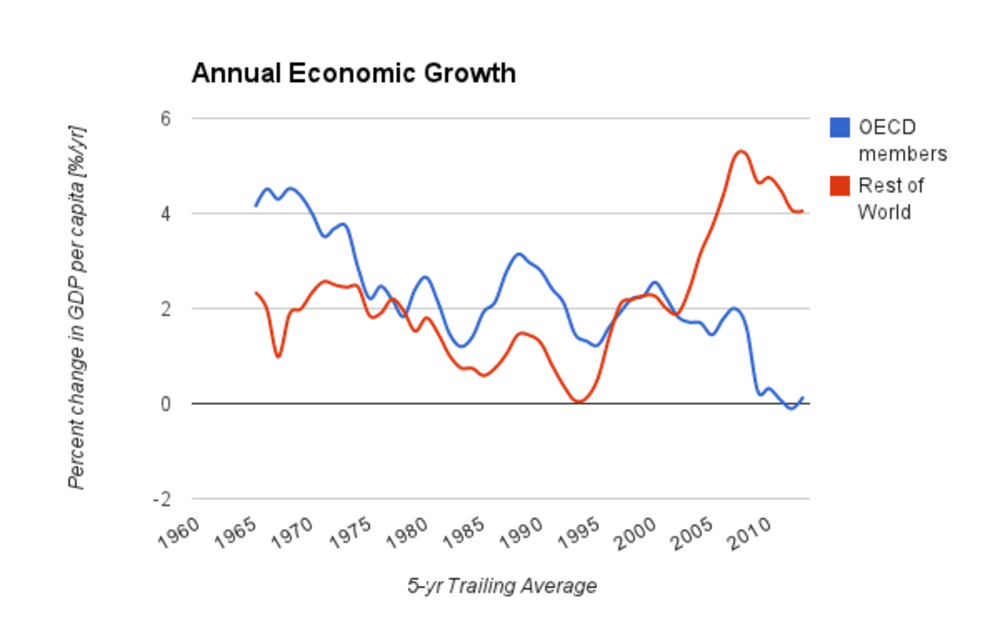
\includegraphics[width=\linewidth]{Part_0/Chapter_Introduction/images/GDPPC.pdf}
\caption[The traditional model]{Source: Authors' calculations using 
data obtained from World Bank databank (Indicator NY.GDP.PCAP.KD.ZG accessed August 1, 2014.)
Source note: ``Annual percentage growth rate of GDP per capita based on constant local currency. Aggregates are based on constant 2005 U.S. dollars. GDP per capita is gross domestic product divided by midyear population. GDP at purchaser's prices is the sum of gross value added by all resident producers in the economy plus any product taxes and minus any subsidies not included in the value of the products. It is calculated without making deductions for depreciation of fabricated assets or for depletion and degradation of natural resources.''}
\label{fig:gdppc}
\end{figure}

The stagnation of economic growth (as measured by percent change in GDP per capita) for mature economies is even more striking when set against the backdrop of the high rates of economic growth of emerging economies. China, India, Indonesia, Brazil, and Russia experienced economic growth rates of 7\% or more over the last fifty years and are expected to maintain relatively high growth rates over the next fifty years. (OECD2014) Figure~\ref{fig:gdppc} shows the average economic growth rates of OECD countries versus the rest of the world since 1960.

Accompanying the slowdown of economic growth in mature economies are poor outcomes along a number of other measures: flat growth rates of median household incomes, high levels of long-term unemployed, and high and increasing levels of public and private debt. Not one of these measures is expected to turn around easily or soon.

What do economists believe is causing this slowdown? Mainstream economic growth theory considers economic growth to be driven by four factors: (1) increased labor utilization through increases in the number of workers or worker hours, (2) increased human capital through improvements in education levels, skill levels, or health, (3) increases in the capital/labor ratio through increases in capital investments, and (4) increased worker productivity through technological innovation. Economist Tyler Cowen argues that large productivity gains through innovation have permanently plateaued leading to a "great stagnation" in economic growth.\cite{Cowen2011}

%*** Mature economies need to come to grips with slowing growth. What might that look like? We have two case studies. The US %and Japan.  In the US, it seems to be tearing at the social fabric. Civic discourse is polarized, with rational dialogue and %response to critical issues made nearly impossible. Political polarization and government dysfunction in the US are a human %response to an economy not producing the growth in incomes that we have become accustomed to.  In contrast, Cowen %argues, the Japanese response  to their country's 25-year economic slump  has been stoic and civil and is a model for the US to %follow. *** (BRH says, I need to either delete or expand this paragraph. Which do you all vote for?)

But, the economy has not only plateaued along the lines of technological innovation. Cato Institute's economic growth specialist, Brink Lindsay, suggests that growth has permanently stalled because all four of the primary drivers of economic growth have plateaued; hours worked, worker skill level, and the amount of capital invested per worker have reached their low, slow steady state and are unlikely to rebound.\cite{lindsay2013} 






%%%%%%%%%% Stalled growth is a problem %%%%%%%%%%
\section{[BRH] Stalling economic growth is a problem}
\label{sec:stall_is_a_problem}
%%%%%%%%%%
Is stalled economic growth a problem? Most analysts believe it is. Past experience suggests that rapid growth in GDP raises living standards and well-being. Various indices of well-being have improved dramatically over the recent centuries. [BRH - flesh out more]

The concern now is that stalled economic growth will continue to be accompanied by a wide spectrum of social ills, including:
\begin{itemize}
	\item{declining living standards}
	\item{inequity}
	\item{high levels of debt}
	\item{unemployment}
\end{itemize}

All of which are being experienced right now as the economy is in its slump. Other aspects of the economy are off-track as well: middle-class incomes of mature economies have stalled. Higher unemployment levels are the new normal. Governments as well as private citizens are running high and increasingly higher levels of debt to maintain the same standard of living.

In all of the discussion about the dismal "new normal," the blame is placed squarely on a slowdown in productivity increases. Thus, the prescribed cure for these ills is to increase economic growth (as measured by percent increase of GDP per capita). This is the only tool policy makers have in their tool kit.

%%%%%%%%%% Stalled growth is a problem %%%%%%%%%%
\section{[BRH] Two alternate views}
\label{sec:stall_is_a_problem}
%%%%%%%%%%
A striking aspect of mainstream economic analyses is that nowhere in the diagnosis of the problem of stalled growth does the economy's reliance on the biosphere play a role. Because the biosphere places physical limits on the economy in terms of (1) material inputs and (2) the energy to run the economic engine, these two binding constraints on economic growth should be a part of models of economic growth. 

Yet, mainstream economic growth models and the policy presecriptions that emerge from them do not identify biophysical limits to the economy as a potential a contributor to the economic downturn. The above analyses from Cowen and Lindsay represent the broad plethora of traditional explanations for the growth slowdown provided by the mainstream. And, the policy prescriptions based on them all call for some way to re-invigorate growth through a variety of traditional means. 

Beyond the economic mainstream, the relationship between the economy and the biosphere is a natural feature of the the intellectual landscape. Thus, beyond the mainstream the analysis of patterns of economic growth and economic downturns can include consideration of biophysical limits. Robert Ayers foretold suggested that the "growth paradigm" would soon come to an end, forcing economies to restructure around renewable energy, closed material cycles, and shifting from goods manufacturing to service provision.\cite{ayers1998} Economics and politics have operated under the assumption that the economy will always continue to grow. A consequence of including the biosphere in economic analysis is a re-emergence of the discussion about a nation's wealth as well as its income. 

[BRH - include a discussion of stock vs. flow]


However, why this is the case and what to do about it is the matter of much debate. 


%%%%%%%%%% Exogenous factors %%%%%%%%%%
\section{[MKH] Exogenous, biophysical factors}
\label{sec:exogenous_factors}
%%%%%%%%%%

As mentioned in Section~\ref{sec:stall_is_a_problem}, 
very little of the discourse 
about mature economy slowdown 
in mainstream economic circles
involves biophysical factors.%
	\footnote{
	In this context, we are using the term ``biophysical factors''
	to indicate any factor related to 
	the extraction, transport, processing, manipulation, and disposal 
	of the physical (as opposed to financial) manifestation 
	of any material or energy resource in the economy.
	}
Mainstream economics considers biophysical factors
to be \emph{exogenous} to the economy.%
	\footnote{
	Of course, mainstream economics discusses \emph{prices}
	of raw materials, goods, and services. 
	And, to the extent that biophysical factors affect prices,
	it could be said that mainstream economic discussions involve
	biophysical factors.
	However, biophysical factors are rarely acknowledged as causal 
	for establishing the prices of goods and services and the raw materials 
	of which they are comprised.
	}

Arguably, the most important (but not the only) biophysical factor 
vis-\`{a}-vis the economy is energy.
If we are to understand how exogenous factors cause economic slowdown
and, conversely, drive economic growth,
we would do well to understand how energy operates in the economy.
Thus, we first discuss the correlation 
between energy consumption and economic activity 
(Section~\ref{sec:energy-economy_coupling}).
Then, we show how economic demands for energy and materials
are related to important stocks 
of raw materials and energy resources in the biosphere 
(Section~\ref{sec:stall_non-renewable_stocks})
and the stocks of manufactured capital in the economy
(Section~\ref{sec:stall_capital_stock}).


%+++++++++ Energy-economy coupling ++++++++++
\subsection{Coupling between energy and the economy}
\label{sec:energy-economy_coupling}
%+++++++++

All manufactured goods are made and services provided
from raw materials that have been
manipulated, processed, transported, or otherwise transformed using energy.
Indeed, energy consumption and economy activity are highly correlated,
as Cleveland, et.\ al.\ showed in a 1984 cover story for \emph{Science}. 
(See Figure~\ref{fig:Cleveland1984}.)

\begin{figure}[!ht]
\centering\
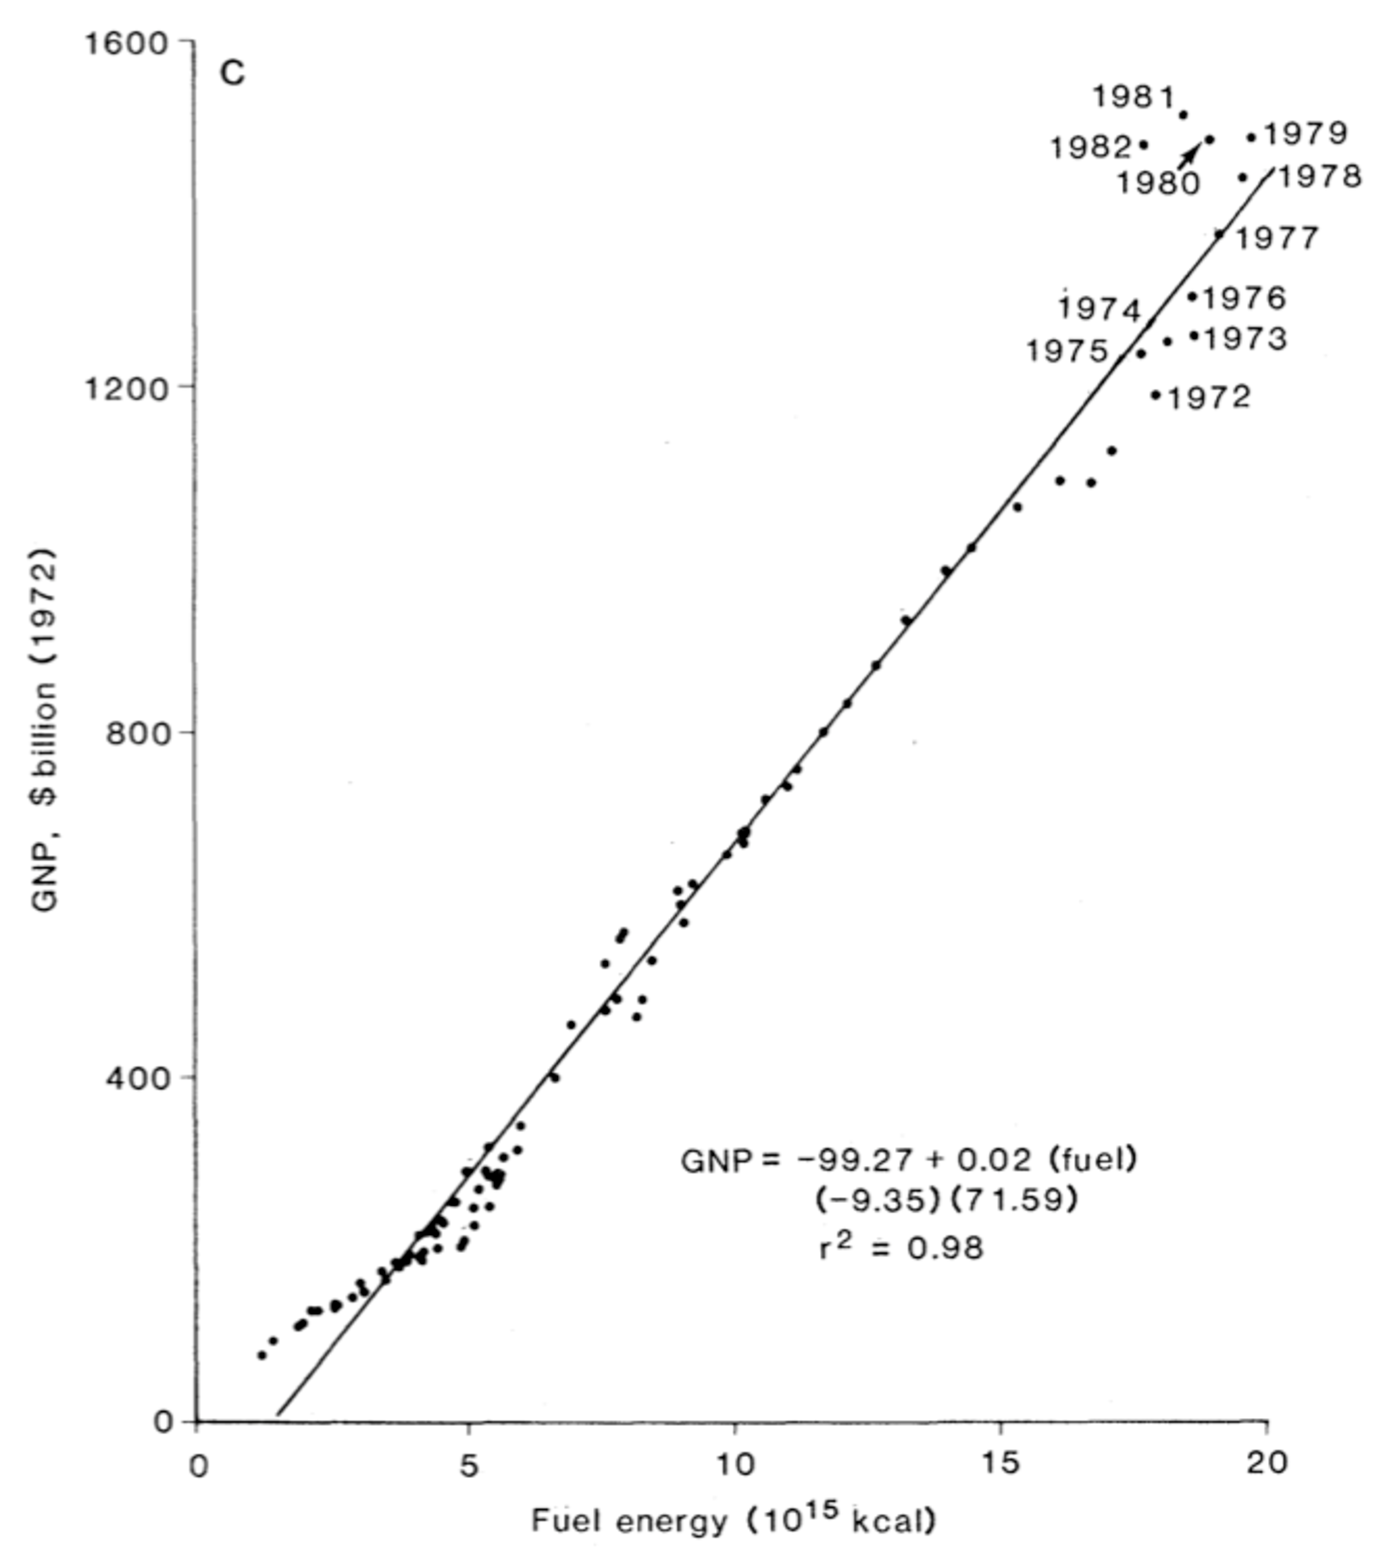
\includegraphics[width=\linewidth]{Part_0/Chapter_Introduction/images/Cleveland1984.pdf}
\caption[Energy and economic activity]{The famous graph from Cleveland, et.\ al.\
\cite{Cleveland:1984aa} showing the strong correlation 
between energy and economic activity from 1890 to 1982.
**** Need to obtain permission to use this graph? ****}
\label{fig:Cleveland1984}
\end{figure}

Because of the high correlation between energy consumption and economic activity,
it stands to reason that energy shortage relative to demand will hinder economic activity.
Of course, there are degrees of shortage. 
In extreme cases, and in the absence of price controls,
goods become hard to find and prices spike
as observed in the US during 1970s oil crisis.
(See Figure~\ref{fig:gas_shortage}.)

\begin{figure}[!ht]
\centering\
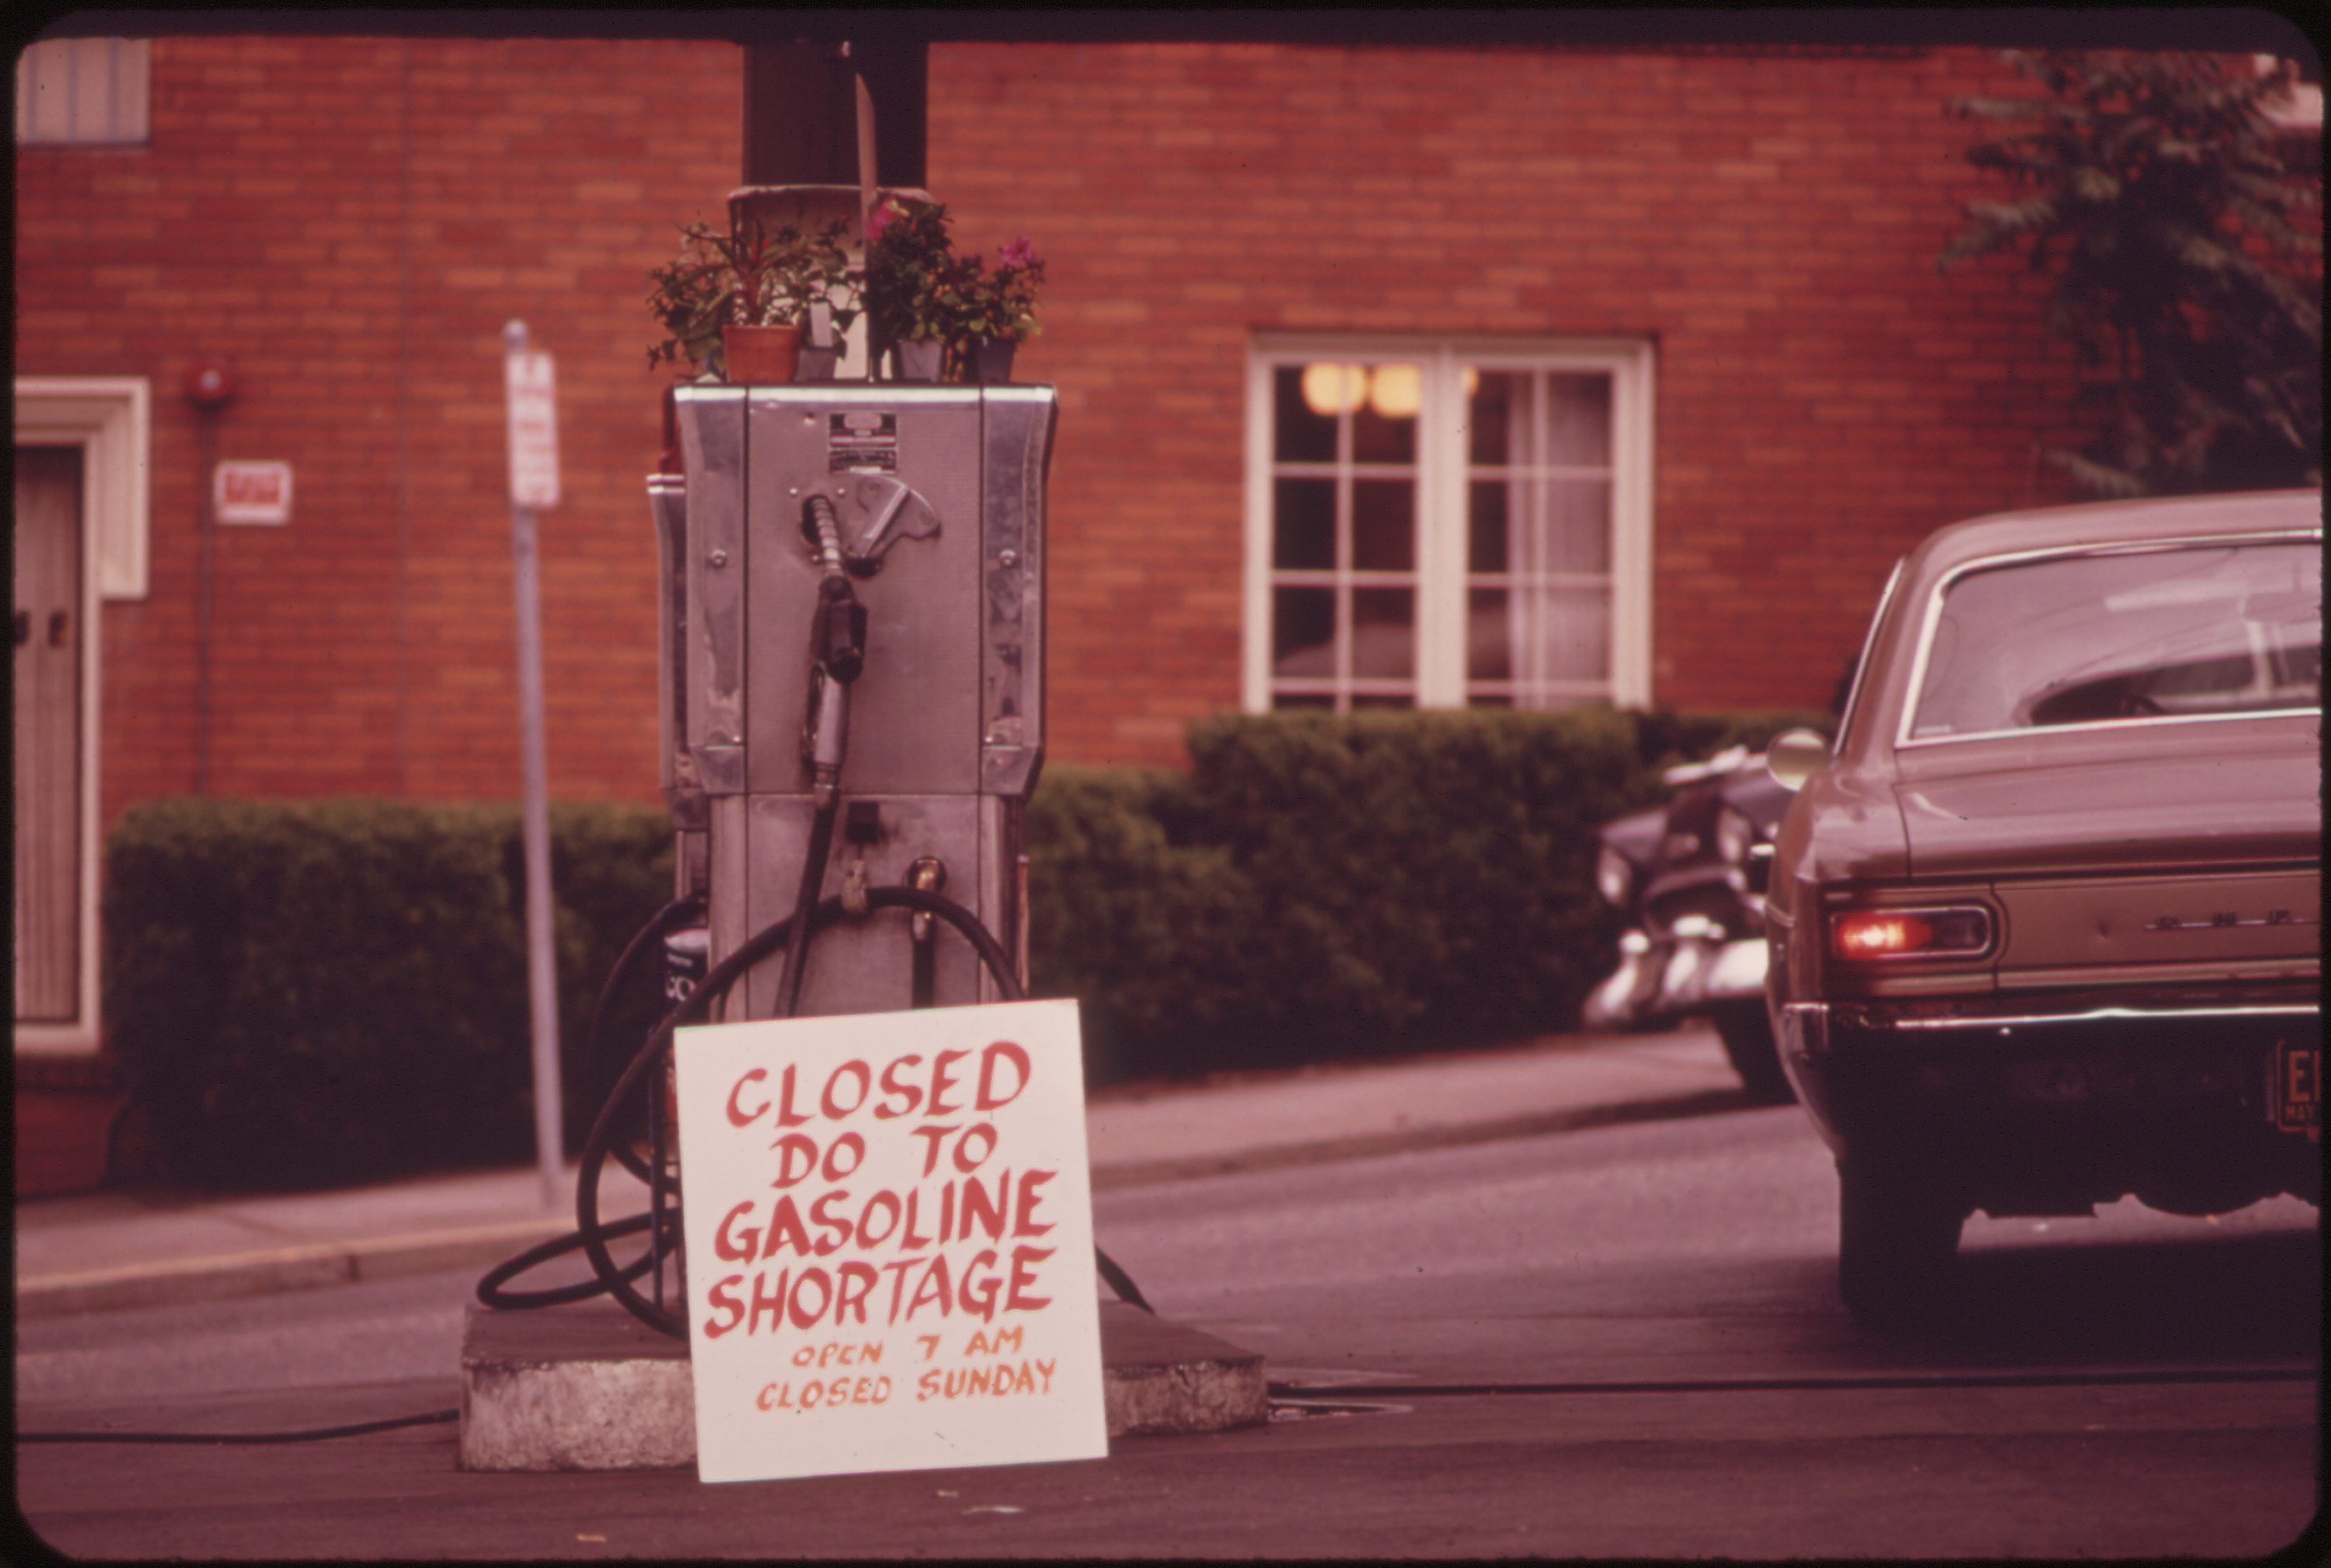
\includegraphics[width=\linewidth]{Part_0/Chapter_Introduction/images/gas_shortage_1973.jpg}
\caption[Gasoline shortage]{Gasoline shortages in 1973.
**** We probably don't need to obtain permission to use this photograph, because
it is from the US national archives.
\url{http://arcweb.archives.gov/arc/action/ExternalIdSearch?id=548053}
\url{https://www.flickr.com/photos/usnationalarchives/4272321708/in/set-72157623204210352/}}
****
\label{fig:gas_shortage}
\end{figure}

In mild cases,
shortage of any good relative to demand leads to rising prices,
even when goods remain available.
For example,
Figure~\ref{fig:oils_prices_and_production} shows oil prices (line) and 
worldwide oil production (vertical bars) 
before, during, and after the great recession. 
Demand for oil increased steadily in the early 2000s
due to worldwide economic growth, 
and production mostly kept pace through early 2005.
However, demand continued to increase while 
production flat-lined from early 2005 through late 2007, 
leading to a steep price increase.
From late 2007 through the end of 2008, 
the small amount of remaining reserve oil production was brought online,
but it was too little, too late.
Prices spiked above \$130/barrel in mid-2007. 
The great recession reduced demand slightly (by about 2 Mb/day)
and the price collapsed to about \$40/barrel.
Thereafter, demand and price rose to their previous levels 
as the world pulled out of the great recession.
In the years since 2008, oil production has risen slightly past the previous record highs
as additional production capacity has come online.

\begin{figure}[!ht]
\centering\
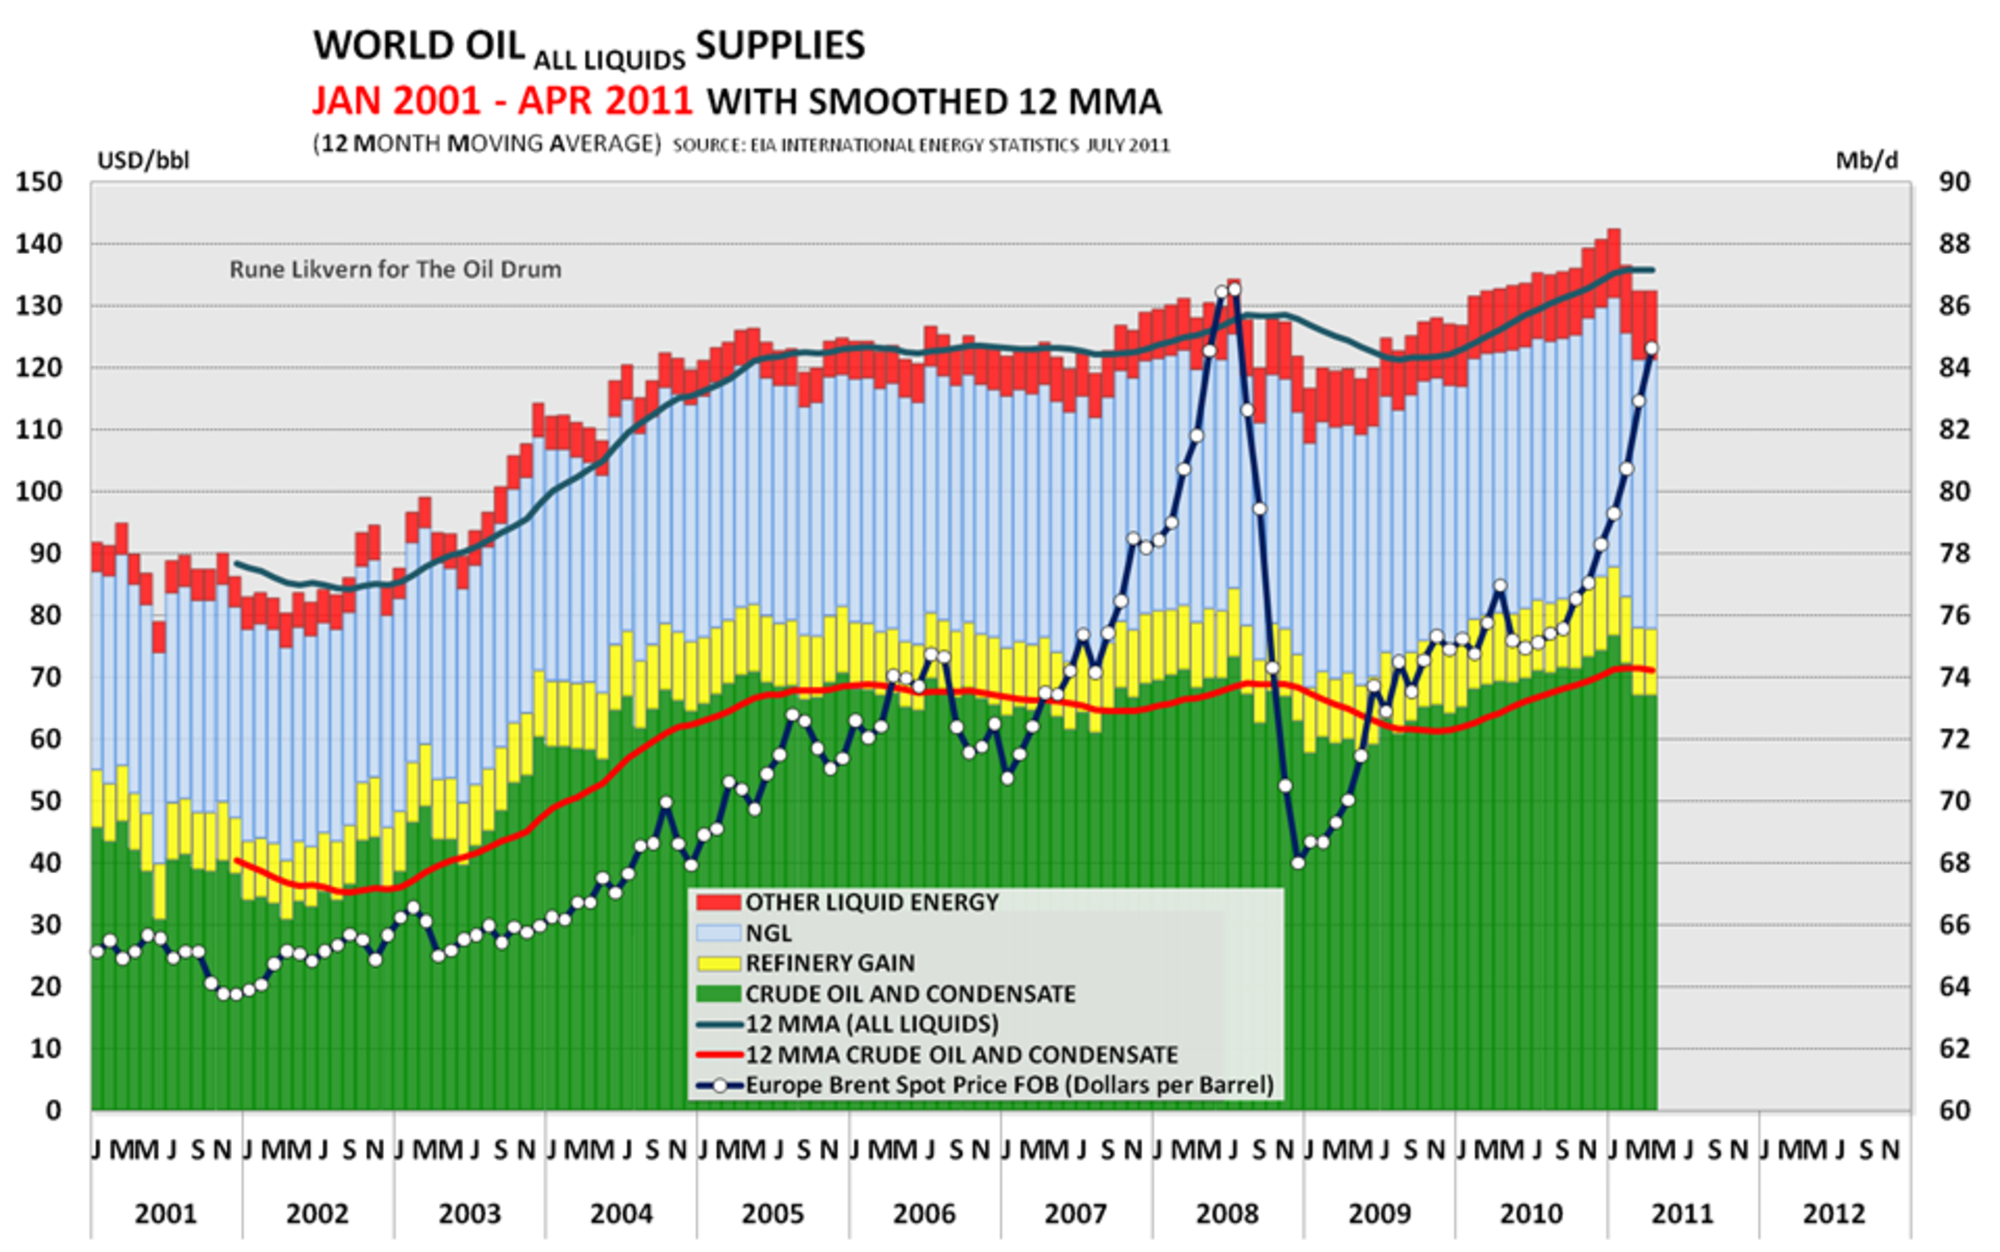
\includegraphics[width=\linewidth]{Part_0/Chapter_Introduction/images/Oil_Prices.pdf}
\caption[Oil prices and production]{Oil prices and production.
**** Recreate this graph from our own data? \url{http://www.theoildrum.com/node/8162}} ****
\label{fig:oils_prices_and_production}
\end{figure}

In both cases (1970s and 2000s), 
significant slowing of economic activity (recessions)
followed the oil shortages and prices spikes.
These were not isolated cases.
Hamilton noted that 
10 of the 11 US postwar recessions 
involved the same pattern.\cite[p.~45]{Hamilton:2013vc}
It is clear that 
there is a correlation between energy consumption and economic activity.

But, what are the dynamics that cause economic slowdowns 
to follow energy price spikes?
When prices rise faster than the cost of production, 
the profit motive should, according to economic theory, induce 
new firms to enter the market and
established firms to increase production.
However, the timing of supply and demand events is crucial.
If firms can't or don't increase production to meet demand, 
prices will remain elevated.
Even without increased production, falling demand will 
bring prices back to earth.

In terms of energy, and oil in particular, 
the \emph{rate} at which production can be increased 
is of the utmost importance, and
there are physical and technological limits. 
Consider this series of thought experiments:
We know that increasing the worldwide oil production rate by, say, 20\% 
involves
finding additional oil deposits, 
drilling additional wells, 
installing new pumps,
and expanding transport and delivery infrastructure worldwide.
In 1960, would it have been possible to achieve such an increase 
over a span of 5 years?
Yes. 
In fact, the worldwide oil production rate increased at a faster rate 
during the 1960s.
There was enough oil in the ground, 
and the economy could absorb the demand 
for additional steel, vehicles, energy, etc.\ required to emplace
the required infrastructure.
The impact on the financial system was minimal, 
because the cost of materials, equipment, labor, and energy
was spread out over a long-enough timeframe (in this thought experiment, 5 years). 
But, in 1960 could worldwide the oil production rate have been increased 
by 20\% in 3 months?
No.
There was enough oil in the ground,
but it would have been practically impossible to manufacture,
transport, and put into service the all the necessary capital in such a short time.
Biophysical constraints limit the rate at which oil production can be increased.
What about 2 years?
Probably not.
It might have been physically possible, 
but the financial cost would have been too much to bear over such a short timeframe,
and the profit motive would be lost.

%Because we don't have infinite time to adjust to biophysical constraints,
This thought experiment shows that time constraints,
layered upon physical and technological constraints, 
are the ties that bind the financial to the biophysical.
Put another way, temporal considerations are the point at which the economy 
becomes coupled to the biosphere.

In economic terms, biophysical constraints reduce the 
price elasticity of supply, the 
percent change in supply for a one percent change in price
during a given period of time.%
	\footnote{
	The mathematical definition of elasticity of supply ($E_s$) is
	\begin{equation*}
		E_s \equiv \frac{\frac{1}{Q}\frac{\partial Q}{\partial t}}
					{\frac{1}{P}\frac{\partial P}{\partial t}} \; ,
	\end{equation*}%
	where $Q$ is quantity of production, $P$ is price, and $t$ is time.
	}
Figure~\ref{fig:oils_prices_and_production} shows that 
a \emph{very large} percentage change in the price of oil was required to 
increase production by only a \emph{very small} percentage
in the 2005--2008 timeframe.
World oil production rose from 
78~million barrels per day to 86~million barrels per day,
an increase of only 10\%.\cite{EIA2014}
However, the inflation-adjusted price of oil increased 260\%,
from around \$35 to a peak of \$126 per barrel 
(in constant 2010 USD).
Thus, the price elasticity of oil supply is very low, about 0.04.
Since 2010, the price of oil has remained over \$80 per barrel,
suggesting that production cannot increase quickly enough relative to demand
to bring prices back down to historical levels.
Persistently high prices for such an important commodity
suggest very real limits to production; 
supply is constrained relative to demand. 

In these circumstances, 
oil supply is said to be very \emph{inelastic} to price.
The observed price inelasticity is caused by 
the biophysical limits to oil production discussed above.
Nothing, not even historically-high prices, can induce producers to 
increase the rate of supply in the short term (say, a 5-year time span), 
because it is physically impossible to do so.
In 2008, the world was running at full oil production capacity, 
but economies demanded more!
Because it was physically impossible to meet that demand,
prices spiked.

But, what caused the recession that followed?
Recently, a few authors have found that \emph{energy cost share},
the fraction of GDP spent on energy, 
is an explanatory variable for these dynamics.
	\footnote{
	Mathematically, energy cost share ($f_E$) is defined as
	\begin{equation}
		f_E \equiv \frac{1}{GDP} \displaystyle\sum_i P_i Q_i \; ,
	\end{equation}
	where 
	the subscript $i$ indicates types of energy 
	(electricity, gasoline, natural gas, etc.),
	$P$ indicates the price of energy,
	$Q$ indicates the quantity of energy purchased within the economy, and
	$GDP$ is gross domestic product.
	}
To our knowledge, 
Bashmakov was the first to 
identify a long-term sustainable range for energy cost share
in mature economies.\cite{Bashmakov:2007ek} 
He also showed that developed economies 
can sustain high total energy cost share
for a short period of time 
(possibly 2--3 years) 
before recessionary pressures 
destroy energy demand,%
	\footnote{
	Note that ``destruction of energy demand'' 
	is accomplished through recession
	in the short run.
	}
stimulate energy efficiency,%
	\footnote{
	Like increasing oil production, 
	increasing energy efficiency also has 
	physical and technological limits.
	Improving energy efficiency is a medium- to long-term process. 
	}
reduce energy prices, 
and return total energy cost share to its long-term sustainable range.
On the other hand, reduction of total energy cost share below 
a lower bound provides economic stimulus, 
increases energy demand, 
provides upward pressure on energy prices, 
and returns energy cost share to its long-term sustainable range.
Bashmakov speculates that 
``energy affordability thresholds and behavioral constants'' 
are responsible for the stable range of energy cost share 
over many decades.\cite[p.~3585]{Bashmakov:2007ek} 
The long-term stable range for economy-wide energy cost share 
(which includes all forms of energy, including oil, natural gas, and electricity)
is 9--11\% for the OECD. 
For oil only, Murphy and Hall found that 
the oil cost share threshold that correlates with US recessions 
is about 5.5\%.\cite{Murphy:2011jh}

The picture emerging from this research shows that 
the cost share of energy in the economy
(and, perhaps more narrowly, oil cost share in the economy)
is an important factor in stimulating or restraining economic growth,
despite its small value (typically, less than 10\%).%
	\footnote{
	Embarking on an economic growth path
	appears to reduce the energy cost share in an economy from very high values
	(indicating that nearly all economic activity is focused on procuring energy)
	to small values that remain within a stable range.
	For example, Sweden's energy cost share has stabilized at 12\% since 1970,
	although it was nearly 100\% in 1800.\cite{Stern:2012ey}.
	}
It appears that the economy-biosphere system has 
a built-in feedback mechanism that 
enforces alignment between biophysical limits and the economy.

This may be somewhat surprising in light of mainstream economic theory, 
which ascribes economic importance 
based on financial cost share, 
not biophysical factors. 
Indeed, the cost share of energy in mature economies is low, 
and viewing energy as relatively unimportant is justified if
one's view of ``importance'' is limited to financial information only.
But, many have noted that the physical importance of energy to the economy 
far exceeds its cost share.\cite{Ayres:2013aa}
And, as discussed above, because the economy is coupled 
to the biophysical world through time constraints (as manifest 
by the low price elasticity of energy supply), 
the physical importance of energy far exceeds its financial importance.

The connection between energy and the economy may be difficult to see, 
but, eventually, it becomes impossible to ignore.


%+++++++++ Stall related to non-renewable stocks ++++++++++
\subsection{[MKH] Stall is related to non-renewable stocks}
\label{sec:stall_non-renewable_stocks}
%+++++++++

Given the tight coupling between the biosphyical world and the economy,
especially regarding energy,
discussed in Section~\ref{sec:energy-economy_coupling} above,
it is prudent to consider the important economic role of
material and energy stocks in the biosphere.

The Best First Principle~\cite{Cleveland:2008aa}
indicates that the economy will extract the easiest-to-obtain 
stocks of mineral and energy resources first.
``Best'' and ``easiest'' can be measured in several ways, 
but it usually comes down to cost.
For example, inexpensive-to-obtain West Texas crude oil was extracted
before expensive-to-obtain offshore oil. 
Surface deposits of gold and diamonds are exhausted before subsurface
veins and kimberlite pipes are exploited.
High-purity mineral deposits are exploited before low-purity deposits.
As a result, it becomes more ``difficult'' to continually increase
extraction rates as time proceeds.
To continue with our energy example,
historical oil production trends reflect these realities.
Through time, the annual rate of increase of oil production
has declined from 7.8\%/year to 0.7\%/year.
(See Figure~\ref{fig:oil_production}.)

\begin{figure}[!ht]
\centering\
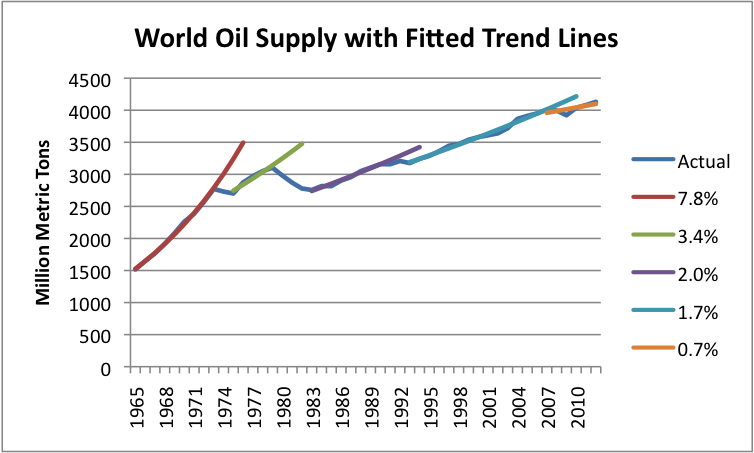
\includegraphics[width=\linewidth]{Part_0/Chapter_Introduction/images/growth-in-world-oil-supply.png}
\caption[World Oil Supply]{Slowing growth in world oil supply.
\url{http://ourfiniteworld.com/2013/10/02/our-oil-problems-are-not-over/}
**** Becky--can you obtain this data and plot it similarly? ****
}
\label{fig:oil_production}
\end{figure}

It is important to realize that it takes energy to make energy available to society.
Oil production requires energy for the ongoing
operation of pumps, 
transportation of crude to the refinery,
refinement of crude to useable petroleum products, and 
transportation of refined products to consumers and firms.
In addition, it takes energy to manufacture the wells, pumps, 
tankers, pipelines, and
refineries used in oil production and distribution.
Furthermore, it takes energy to use energy. 
The economy uses energy to manufacture the machines (vehicles, mostly)
that consume refined oil products.

Application of the Best First Principle to the energy production process 
indicates that it will take more energy 
to make energy available to society as natural energy resources are depleted.
The metric that measures the energy impacts of the Best First Principle is 
Energy Return on Investment ($EROI_{soc}$), 
the ratio of energy provided to society 
by the energy consumed in making it available.%
	\footnote{
	Energy return on investment ($EROI_{soc}$) at the societal level is defined as 
	%
	\begin{equation}
		EROI_{soc} \equiv \frac{\dot{E}_a}{\dot{E}_c} \; ,
	\end{equation}
	%
	where $\dot{E}_a$ is the rate of energy made available to society in MJ/year
	and $\dot{E}_c$ is the rate of energy consumed in the energy production process in MJ/year.
	}
As energy resources in the biosphere are depleted, 
the Best First Principle entails that
$EROI_{soc}$ will decline.
Indeed it has.
Turning again to our oil example, $EROI_{soc}$ for oil has declined 
from a value of 100 in the 1930s~\cite[p.~781]{Cleveland:2005uy} 
to around 20 today.\cite[Fig.~2]{Hall:2014aa}
In other words, it takes 5~times more energy today
than it did in 1930
to make a barrel of oil available to society.

Furthermore, declining $EROI_{soc}$ for oil has economic impacts.
Both Heun and de~Wit~\cite{Heun:2012ek} and King and Hall~\cite{King:2011go}
show that declining $EROI_{soc}$ correlates with higher prices for oil, 
because declining $EROI_{soc}$ provides upward pressure on 
production costs, and therefore, prices
as time proceeds.

All other things being equal, the Best First Principle
indicates that the additional physical ``effort'' required to extract
increasingly-marginal resources will lead to decreased extraction rates.
In the race against the Best First Principle,
technological advances can bring about higher extraction rates, 
despite the additional physical ``effort'' required.

**** BRH: Talk about Ricardo here? ****

For example, the recent shale oil boom, made possible by new extraction technology,
has increased US oil production significantly. 
But, Figure~\ref{fig:US_oil_production} shows that increased US production
is due to so-called ``tight'' oil (which includes shale oil), 
that has lower $EROI_{soc}$ than crude oil.
Furthermore, today's ``tight'' oil is more expensive to produce 
than the crude of yesteryear.
Consequently, oil prices must remain high for 
shale oil production to remain financially feasible into the foreseeable future. 
Unfortunately, Section~\ref{sec:energy-economy_coupling} indicates that
high energy prices can lead to high energy cost share in the economy
and recessionary pressures.

\begin{figure}[!ht]
\centering\
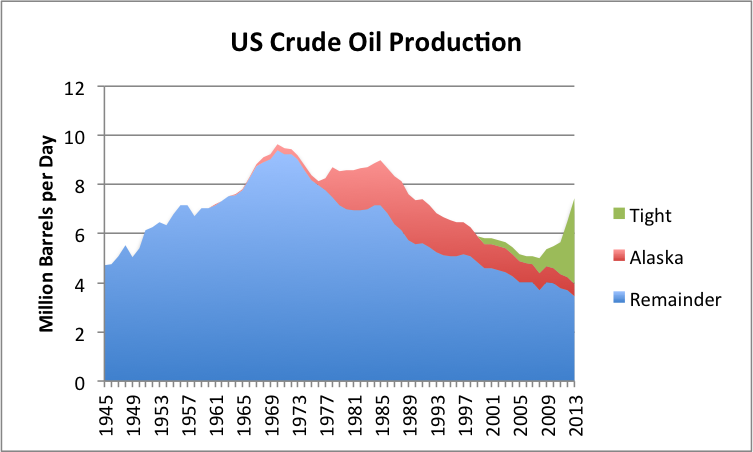
\includegraphics[width=\linewidth]{Part_0/Chapter_Introduction/images/us-crude-oil-production-including-tight-oil.png}
\caption[US oil production]{US oil production.
\url{http://ourfiniteworld.com/2014/07/23/world-oil-production-at-3312014-where-are-we-headed/}
**** Becky--can you obtain this data and plot it similarly? ****
}
\label{fig:US_oil_production}
\end{figure}

The fact that shortages of crude oil provide incentives for 
technological advancements that bring new production online (e.g., shale oil)
appears, at first glace, to be a good thing.
However, energy substitutions are beneficial to society 
in the long run only when the $EROI_{soc}$ of the substitute
is equal to or higher than the original.
Thus, the benefits of shale oil are modest, at best, when the
high financial and energy costs of production are considered.

That said, a transition to new sources of energy will be a feature 
of the economy in the age of resource depletion.
But, there is evidence of limits to energy substitution 
at the macroeconomic level.
Pelli, in a study of 21 countries 
found that clean%
	\footnote{
	Nuclear, 
	conventional hydroelectric power, wood and waste biomass, 
	geothermal, solar/photovoltaic, and wind
	}
and dirty%
	\footnote{
	Coal, 
	petroleum, natural gas, and other gasses
	}
inputs to electricity production
are complementary (as opposed to substitutable).\cite{Pelli:2012wv}
His conclusion is dire:
%
\begin{quote}
	On the one hand, according to the model, 
	if we keep producing electricity using dirty inputs, 
	we head toward an environmental disaster. 
	On the other hand, looking at the empirical results, 
	it seems impossible to stop producing electricity with polluting resources. 
	The policy implication of this paper thus, 
	seems to be that we need more important subsidies to research, 
	as fast as possible, 
	and high carbon taxes combined with a complete halt 
	of the growth rate of the production of electricity. 
	In this way, according to the model, 
	we may be able to avoid an environmental disaster.\cite[p.~25]{Pelli:2012wv}
\end{quote}

In a meta-analysis of 15 papers that studied 
the economic evidence for macro-substitutability
among factors of production (materials, capital, labor, and energy), 
de Wit et.\ al.~\cite{de-Wit:2013aa} found that the elasticity of substitution was 
below unity for all combinations of factors of production.
Furthermore, they argue that, 
%
\begin{quote}
	[because all of the] results show elasticity of substitution below unity, 
	none of the factor inputs are perfectly substitutable and 
	all tend toward complementarity in varying degrees. 
	Such results suggest that transitions 
	from one production or consumption structure to another 
	can be disruptive and that the transitions 
	need to be modeled dynamically to the extent possible.\cite[p.~8]{de-Wit:2013aa}
\end{quote}

The challenges of energy substitutions are highlighted
when examining the financial situation of oil producers.
Figure~\ref{fig:oil_company_free_cash_flow} 
shows that despite the recent increase in oil production
and continued high prices, 
the free cash flow of independent oil producers is negative.
It remains to be seen how independent producers can continue advancing 
production without free cash flow to cover capital expenditures.
One possible cure is higher oil prices.
But, again, we saw 
in Section~\ref{sec:energy-economy_coupling}
that high energy cost share 
provides recessionary pressure.

\begin{figure}[!ht]
\centering\
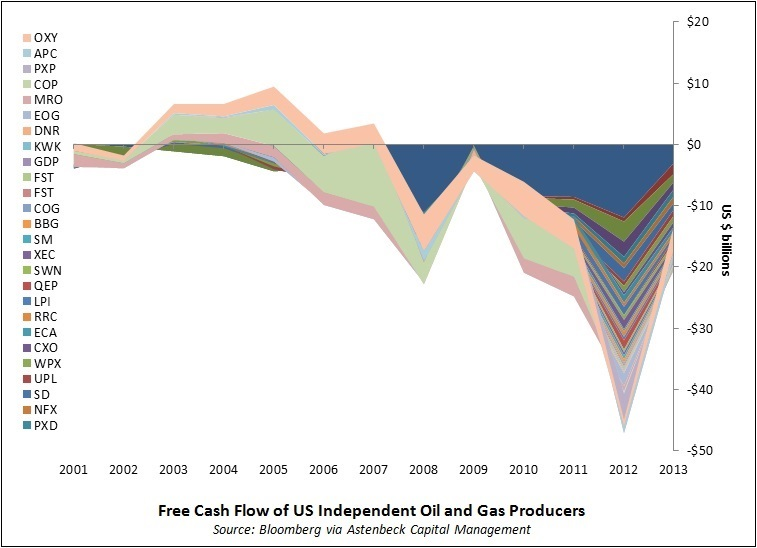
\includegraphics[width=\linewidth]{Part_0/Chapter_Introduction/images/Cash-Flow.jpg}
\caption[Oil company free cash flow]{Oil company free cash flow.
\url{http://blogs.platts.com/2014/07/30/peak-oil-forecasts/}
**** Becky--can you obtain this data and plot it similarly? ****
}
\label{fig:oil_company_free_cash_flow}
\end{figure}

All of this comes about simply because it is 
more physically ``difficult,'' and, as a consequence, 
more financially expensive
to extract oil today than it was 10, 20, 30, and 100 years ago.
It is more difficult to obtain oil today because we have depleted
the stocks of easy-to-obtain crude oil from the biosphere.
And, the remaining stocks are either lower quality (e.g., shale)
or further away (e.g., deeper offshore).

Without going into detail, we state without discussion 
that similar dynamics will apply to 
any non-renewable material or energy stock in the biosphere
for which substitution is difficult.
Using oil as our example, we observe that 
stocks of natural capital, especially energy resources,
have significant economic implications.
Both the declining \emph{quantity} and 
the diminishing \emph{quality} of remaining non-renewable biosphere stocks 
are contributing to the slowdown of growth in mature economies
discussed in Section~\ref{sec:growth_has_slowed}.

Stocks of another sort also play a role 
in the slowdown of growth experienced by mature economies,
because they  are important drivers of material and energy consumption.
In the next section, we turn our attention 
away from the biosphere 
toward the economy and its stock of capital.



**** [bonepile?] The implication is that solving the resource efficiency problem
is the key to continued growth. [Reference Thomas Friedman here,
\url{http://www.nytimes.com/2012/03/04/opinion/sunday/friedman-take-the-subway.html?hp&_r=0}]
****


%+++++++++ Stall related to capital stock ++++++++++
\subsection{Stall is related to capital stock}
\label{sec:stall_capital_stock}
%+++++++++

The word ``capital'' is used in many ways, usually referring to assets
of one form or another: 
financial capital, 
natural capital, 
human capital, 
social capital,
physical capital, and
manufactured capital, 
to name a few.
In this book, 
we use the term ``capital'' to indicate things such as
machines, 
buildings, 
roads,
vehicles, and
computers,
all physical items used in and necessary for the production process.
Capital is not normally used up during production 
of goods and rendering of services, 
although it depreciates over time.
Capital is extremely valuable and, in most cases, essential to production processes:
machines reduce per-unit costs of production;
buildings provide space to work and protection for capital;
roads provide networks for vehicular transport 
of raw materials, finished goods, and capital itself; and
computers enhance the efficiency of workers and enable technological breakththroughs.
We use the word ``stock'' to indicate the total inventory of capital 
in the economy at a given point in time.

There are several types of capital flows
to and from its stock in the economy.
We use the term ``emplacement'' to denote a flow of capital into
the economy, for example when a new machine is put into service,
when a new building is constructed, or
when a new road is opened.
``Depreciation'' is normal wear-and-tear experienced by capital, 
a type of outflow of capital from the economy.
Financial depreciation involves the write-off of a percentage 
of the value of capital.
Physical depreciation involves wear and tear of parts within or sections of the capital.
Financial depreciation usually occurs faster than physical depreciation.
``Maintenance'' is servicing of capital to overcome the effects of physical depreciation.
``Disposal'' is the physical outflow of capital from the economy to the biosphere
upon removal from service.
Capital ``formation'' is the rate of net
addition to capital stock in the economy,
the difference between inflows and outflows
during a time interval.
Traditionally, stocks and flows of capital are measured by currency units, 
\$ and \$/year, respectively.
However, we argue later (Section~\ref{sec:Implications_for_IO})
that a physical basis for capital accounting is also warranted.

It is important to note that it takes materials and energy
to manufacture and emplace capital at its point of use.
Furthermore, once emplaced,
capital consumes energy to process raw materials 
into intermediate and finished products
and for its maintenance.
The energy required to manufacture and emplace capital
(including all upstream processes)
is called \emph{embodied} energy.
In addition to capital, energy is embodied in all manufactured materials and
products.%
	\footnote{
	See Chapter~\ref{chap:embodied_energy} for more details
	on embodied energy.
	}
The ratio of energy embodied in products to their price 
is the energy \emph{intensity} of output ($\varepsilon$, 
in units of J/\$).%
	\footnote{
	See Chapter~\ref{chap:intensity} for more details 
	on energy intensity.
	}
Both embodied energy and energy intensity are key metrics 
for understanding the economy.
To first order, energy embodied in capital provides an estimate of the 
energy needed for replacement.
The distribution of energy intensity
across products and sectors
provides a picture of energy demands caused by consumption.

Most capital (especially machines) is considerably more expensive
than the individual products it makes.
So, it takes significant financial resources (relative to sales) 
to purchase and emplace capital.
Capital is so beneficial (i.e., productive in the economic sense), 
that firms pursue and obtain debt financing to cover large capital expenses.
In the case of public goods like roads, bridges, and utilities,
governments pursue debt financing via municipal bonds.
The long-term financial obligations associated with capital financing 
mean that the capital is expected to be in service
for at least the repayment period of the debt,
usually much longer.

The long-term commitment to capital and production means that 
emplacement of capital is a bond, a claim on future
raw material and energy \emph{consumption}.
And, it is an assurance of raw material and energy \emph{extraction} 
from the biosphere for many years to come.
Furthermore, extant productive capital stock can't be fed just any material or energy;
capital is designed to work with only certain types of materials and energy.
An auto body panel stamping machine is designed to form steel, perhaps even a specific 
grade or alloy of steel;
feeding plastic won't do.
The machine likely runs on electricity; 
feeding gasoline won't do.

Thus, the stock of capital in the economy 
is an important driver of not only 
the rate but also  
the type of
material and energy flows from the biosphere.
The emplacement of productive capital
``locks in'' demand for specific types of materials and energy 
into the forseeable future.
As such, long-term commitments associated with emplaced capital
provide limits to the rate at which society can effect
transitions to different raw materials and energy sources.
Again, we observe tight coupling between the economy and the biosphere!

Given the discussion in Section~\ref{sec:stall_non-renewable_stocks}
	regarding the economic dynamics 
	of biophysical limits to raw material and energy extraction,
	we see that, paradoxically, and contrasting with all mainstream policy prescriptions
	(see Section~\ref{sec:policy_flows}), 
	expansion of the stock of capital in the economy 
	is another factor that could contribute to the slowdown of economic growth.

\begin{svgraybox}
	Expansion of an economy's  capital stock may increase GDP
	in the short run. But, it also ``locks in'' 
	future material and energy demands 
	from the biosphere.
	These bring the economy closer 
	to the biophysical extraction limits 
	that will eventually lead to economic slowdown.
\end{svgraybox}


%%%%%%%%%% Consumption-driven policies are unsustainable %%%%%%%%%%
\section{[ BRH, MKH] Consumption-driven solutions are unsustainable}
\label{sec:consumption_unsustainable}
%%%%%%%%%%
Biophysical limits to economic growth are becoming a binding constraint, thus 
increases in manufactured capital stock
can ultimately lead to economic slow down. The cost benefit analysis
related to capital stock investment decisions not only 
includes the opportunity cost of the next best alternative investment in manufactured capital, 
but also the net present value of all future demands on natural capital. Those
costs need to be considered as part of the analysis at the firm, industry, and economy
levels.

In Section~\ref{sec:stall_capital_stock} above, 
we noted that existing policy designed to combat economic slowdown 
in mature economies is focused on 
increasing many material, energy, and financial flow rates in the economy.
Set against the backdrop of Section~\ref{sec:exogenous_factors},
we see that consumption-driven policies are ineffective,
because of biophysical limits that constrain the scale of the economy. 
Unfortunately, biophysical limits 
are not included in the mainstream economic thinking and modeling
that informs policy decisions.%
	\footnote{
	More on the problematic nature of this issue
	can be found in Section~\ref{sec:metaphors_and_models}.
	}

Three factors, in combination, are vitally important 
but nearly-always ignored:

\begin{itemize}
	\item{the economy is tightly coupled to the biosphere,}
	\item{there are physical and technological limits 
			to the rate at which materials and energy can be extracted 
			from the biosphere, and}
	\item{today's emplacement of capital locks in
			tomorrow's material and energy demands 
			for both operation and maintenance of that capital.}
\end{itemize}

In short, the economic analyses that support 
consumption-driven policies are incomplete.
Consumption-driven economic growth is unsustainable.


%%%%%%%%%% Don't understand real economy %%%%%%%%%%
\section{[MKH] Change is needed!}
\label{sec:change_needed}
%%%%%%%%%%

The fact that we (as a society) do not include exogenous, biophysical factors 
in economic decision-making indicates that
we do not fully understand how the real economy operates.
Society is ignorant of the role that natural and manufactured%
	\footnote{
	Manufactured capital presupposes the existance of 
	significant levels of human and social capital.
	}
capital plays in both sustaining today's economy and 
constraining future economic prospects and choices.
**** The remainder of this paragraph may go better in Becky's section above. ****
One way to measure such policies is to calculate a flow-to-stock ratio,
an indication of the rates of natural resource extraction relative to 
the level of remaining stock.
Policies that aim for high financial flow rates have concommitant high
natural resource flow rates and high flow-to-stock ratios.
**** Reference to Daly or someone else here? ****
Economies with consumption-enhancing policies and high flow-to-stock ratios
are more likely to deplete natural resources due to unsustainable extraction rates, 
because there is little incentive to protect or invest in natural capital. 
As a result, we end up consuming manufactured and natural capital (wealth) 
in the hopes of generating income!

% At present, the market is virtually the only tool at our disposal
% to help us understand the characteristics of the real economy.
% Is the market able to answer these important questions?
%
% \begin{enumerate}
% 	\item{\label{itm:scale}What is the appropriate scale (size) for the economy relative
% 			to the biosphere?---No.
% 			Scale is a non-market issue.
% 			In any case, economic policy-making ignores the biosphere.
% 			(See Section~\ref{sec:metabolic_scale}.)}
% 	\item{\label{itm:distribution}**** delete? **** We only account for things that are owned. BRH try to fix. What is the optimal distribution
% 			of natural capital ownership
% 			(public, private, etc.)?---No.
% 			Ownership of natural resources is a non-market issue.}
% 	\item{\label{itm:allocation}How should products be allocated to final demand?---Maybe.
% 			Competitive markets allocate efficiently, but
% 			we argue that efficiency should be understood in the context of questions
% 			\ref{itm:scale} and \ref{itm:distribution} above,
% 			which markets are unable to answer.
% 			If markets are to be helpful,
% 			they require correct and complete information, and
% 			values of non-market transactions must be available
% 			to market participants.
% 			Such data are unavailable at this time.}
% \end{enumerate}

At present, markets are virtually the only tool at our disposal
to help us understand the characteristics of the real economy.
What benefits do markets provide?
Markets are extremely efficient allocators of resources.
Mainstream economic theory holds that prices are the mechanism by which signals
of value are communicated to sellers and buyers:
sellers receive information about how goods are valued by consumers, and
buyers receive information about the cost of materials accrued by producers.

In the age of resource depletion, 
are price signals sufficient to indicate shortages, 
especially of important and difficult-to-substitute resources?
It appears that some signals are getting through.
Heun and de Wit **** add reference here **** 
showed that scarcity (as indicated by low $EROI_{soc}$)
correlates with higher oil prices.
And, higher prices spur efficiency improvements. 
**** reference here about higher average fuel economy of autos in the US. ****

However, the market's price mechanism may not be enough.
We showed in Section~\ref{sec:energy-economy_coupling}
that the physical importance 
of scarce and difficult-to-substitute resources (e.g., oil) 
far exceeds cost share in the economy,
suggesting that prices alone cannot provide comprehensive
signals of importance to producers and consumers.
Consequently, producers and consumers participate in the market with incomplete information.
Furthermore, a good must be owned before 
it can be sold.
Thus, prices cannot be set and market value cannot be determined
for goods that are not considered ``property,'' 
such as clean water, clean air, and other ``ecosystem services.''
In addition, today's markets are simply incapable of deciding
important issues such as the optimal scale (size) of the economy
relative to the biosphere. (See Section~\ref{sec:metabolic_scale}.)
Because the allocative efficiency of markets is predicated upon 
correct and complete information being available to market participants,
today's markets are a poor choice for allocative decisions about
scarce and difficult-to-substitute resources (such as oil)
or non-property goods (such as clean air, clean water, and other ecosystem services).

In the age of resource depletion, 
the allocative efficiency of markets is attractive.
Indeed, life would be better if the markets could shift supply and demand 
away from binding biophysical constraints
when they are encountered.
But, lack of information in \emph{today's} markets
leads us to argue that they
are not up to the task.

What additional information would be helpful?
We contend that detailed information about energy, embodied energy, and energy intensity
would be a good place to start.
We, as a society, routinely account and publish energy flow rates only.%
	 \footnote{
	 Energy consumption rates are routinely published by the 
	 US Energy Information Agency (EIA) and the 
	 International Energy Agency (IEA).
	 }
We do not, however, routinely update energy \emph{intensity}%
	\footnote{
	Estimates of energy intensity are not included in systems of national accounts.
	And, such work is rarely undertaken by academics.\citep{Bullard1975, EIOLCA2014} 
	}
estimates ($\varepsilon$)
and, therefore, 
we have little idea of where energy is embodied 
in our capital stock and 
in the products we consume.
Furthermore, when energy intensity ($\varepsilon$) of products is estimated, 
it does not account for the energy embodied in our stock of capital
and is therefore in error.%
	\footnote{
	See Section~\ref{sec:Implications_for_IO} for our suggested remedy.
	}
	
We suggest that all of this information 
(economic, material, and energy indicators) 
should be collated by a single agency and
reported from a single location.
Doing so will provide convenience and
indicate the interconnectness of the economy and the biosphere
to policymakers and researchers.

Until these crucial pieces of information are routinely available 
in a centralized location, 
society will be unable to properly frame and conceptualize 
the ``problem'' of ``stalling'' growth. 
Until this information is available to markets,
society will be unable to adequately manage economies.


%%%%%%%%%% Prescriptions worse than disease %%%%%%%%%%
\section{[MKH] Prescriptions may be worse than the disease}
\label{sec:prescriptions_disease}
%%%%%%%%%%

In the end,
our prescriptions for curing slow economic growth 
may be worse than the disease.
**** Maybe combine the rest of this paragraph with Becky's 
section above. ****
Stimulating the economy via consumption-enhancing policies through investments 
in capital stock 
can increase economic throughput (GDP) for a time.
Unfortunately, such policies also
hasten the day when we reach binding biophysical constraints
due to resource depletion. 
Adoption of these policies when society is already encountering
resource depletion constraints
will result in see-saw economic performance. 
In fact, we may have already entered a regime of boom-bust economic dynamics,
because of a binding constraint for oil extraction rate
as discussed in Section~\ref{sec:exogenous_factors}.
In the face of see-saw dynamics,
it is difficult to make wise long-term investment or policy decisions,
because you're perpetually recovering from the most-recent bust.

In the age of resource depletion, 
these dynamics should cause us to measure and report
the material and energy demands that products and capital stock 
make upon the biosphere.
We should know these factors 
in \emph{physical} as well as financial terms,
for constraints of the physical world 
lead to problems in the economy.
These data should be available routinely from a centralized location.

This is the end of an era.
In mature economies, consumption-enhancing 
economic policies can no longer guarantee 
growth of living standards and well-being.
But, the mainstream is blind to what should be done instead. 
This has to change!


\bibliographystyle{unsrt}
\bibliography{../../Metabolic}


% Always give a unique label
% and use \ref{<label>} for cross-references
% and \cite{<label>} for bibliographic references
% use \sectionmark{}
% to alter or adjust the section heading in the running head
%% Instead of simply listing headings of different levels we recommend to let every heading be followed by at least a short passage of text. Furtheron please use the \LaTeX\ automatism for all your cross-references and citations.

%% Please note that the first line of text that follows a heading is not indented, whereas the first lines of all sequent paragraphs are.

%% Use the standard \verb|equation| environment to typeset your equations, e.g.
%
%% \begin{equation}
%% a \times b = c\;,
%% \end{equation}
%
%% however, for multiline equations we recommend to use the \verb|eqnarray|
%% environment\footnote{In physics texts please activate the class option \texttt{vecphys} to depict your vectors in \textbf{\itshape boldface-italic} type - as is customary for a wide range of physical jects.}.
%% \begin{eqnarray}
%% a \times b = c \nonumber\\
%% \vec{a} \cdot \vec{b}=\vec{c}
%% \label{eq:01}
%% \end{eqnarray}

%% \section{section Heading}
%% \label{sec:2}
%% Instead of simply listing headings of different levels we recommend to let every heading be followed by at least a short passage of text. Furtheron please use the \LaTeX\ automatism for all your cross-references\index{cross-references} and citations\index{citations} as has already been described in Sect.~\ref{sec:2}.

%% \begin{quotation}
%% Please do not use quotation marks when quoting texts! Simply use the \verb|quotation| environment -- it will automatically render Springer's preferred layout.
%% \end{quotation}


%% \section{section Heading}
%% Instead of simply listing headings of different levels we recommend to let every heading be followed by at least a short passage of text. Furtheron please use the \LaTeX\ automatism for all your cross-references and citations as has already been described in Sect.~\ref{sec:2}, see also Fig.~\ref{fig:1}\footnote{If you copy text passages, figures, or tables from other works, you must obtain \textit{permission} from the copyright holder (usually the original publisher). Please enclose the signed permission with the manucript. The sources\index{permission to print} must be acknowledged either in the captions, as footnotes or in a separate section of the book.}

%% Please note that the first line of text that follows a heading is not indented, whereas the first lines of all sequent paragraphs are.

% For figures use
%
%% \begin{figure}[b]
%% \sidecaption
% Use the relevant command for your figure-insertion program
% to insert the figure file.
% For example, with the option graphics use
%% \includegraphics[scale=.65]{figure}
%
% If not, use
%\picplace{5cm}{2cm} % Give the correct figure height and width in cm
%
%% \caption{If the width of the figure is less than 7.8 cm use the \texttt{sidecapion} command to flush the caption on the left side of the page. If the figure is positioned at the top of the page, align the sidecaption with the top of the figure -- to achieve this you simply need to use the optional argument \texttt{[t]} with the \texttt{sidecaption} command}
%% \label{fig:1}       % Give a unique label
%% \end{figure}


%% \paragraph{Paragraph Heading} %
%% Instead of simply listing headings of different levels we recommend to let every heading be followed by at least a short passage of text. Furtheron please use the \LaTeX\ automatism for all your cross-references and citations as has already been described in Sect.~\ref{sec:2}.

%% Please note that the first line of text that follows a heading is not indented, whereas the first lines of all sequent paragraphs are.

%% For typesetting numbered lists we recommend to use the \verb|enumerate| environment -- it will automatically render Springer's preferred layout.

%% \begin{enumerate}
%% \item{Livelihood and survival mobility are oftentimes coutcomes of uneven socioeconomic development.}
%% \begin{enumerate}
%% \item{Livelihood and survival mobility are oftentimes coutcomes of uneven socioeconomic development.}
%% \item{Livelihood and survival mobility are oftentimes coutcomes of uneven socioeconomic development.}
%% \end{enumerate}
%% \item{Livelihood and survival mobility are oftentimes coutcomes of uneven socioeconomic development.}
%% \end{enumerate}


%% \paragraph{paragraph Heading} In order to avoid simply listing headings of different levels we recommend to let every heading be followed by at least a short passage of text. Use the \LaTeX\ automatism for all your cross-references and citations as has already been described in Sect.~\ref{sec:2}, see also Fig.~\ref{fig:2}.

%% Please note that the first line of text that follows a heading is not indented, whereas the first lines of all sequent paragraphs are.

%% For unnumbered list we recommend to use the \verb|itemize| environment -- it will automatically render Springer's preferred layout.

%% \begin{itemize}
%% \item{Livelihood and survival mobility are oftentimes coutcomes of uneven socioeconomic development, cf. Table~\ref{tab:1}.}
%% \begin{itemize}
%% \item{Livelihood and survival mobility are oftentimes coutcomes of uneven socioeconomic development.}
%% \item{Livelihood and survival mobility are oftentimes coutcomes of uneven socioeconomic development.}
%% \end{itemize}
%% \item{Livelihood and survival mobility are oftentimes coutcomes of uneven socioeconomic development.}
%% \end{itemize}

%% \begin{figure}[t]
%% \sidecaption[t]
% Use the relevant command for your figure-insertion program
% to insert the figure file.
% For example, with the option graphics use
%% \includegraphics[scale=.65]{figure}
%
% If not, use
%\picplace{5cm}{2cm} % Give the correct figure height and width in cm
%
%% \caption{Please write your figure caption here}
%% \label{fig:2}       % Give a unique label
%% \end{figure}

%% \runinhead{Run-in Heading Boldface Version} Use the \LaTeX\ automatism for all your cross-references and citations as has already been described in Sect.~\ref{sec:2}.

%% \runinhead{Run-in Heading Italic Version} Use the \LaTeX\ automatism for all your cross-refer\-ences and citations as has already been described in Sect.~\ref{sec:2}\index{paragraph}.
% Use the \index{} command to code your index words
%
% For tables use
%
%% \begin{table}
%% \caption{Please write your table caption here}
%% \label{tab:1}       % Give a unique label
%
% For LaTeX tables use
%
%% \begin{tabular}{p{2cm}p{2.4cm}p{2cm}p{4.9cm}}
%% \hline\noalign{\smallskip}
%% Classes & class & Length & Action Mechanism  \\
%% \noalign{\smallskip}\svhline\noalign{\smallskip}
%% Translation & mRNA$^a$  & 22 (19--25) & Translation repression, mRNA cleavage\\
%% Translation & mRNA cleavage & 21 & mRNA cleavage\\
%% Translation & mRNA  & 21--22 & mRNA cleavage\\
%%Translation & mRNA  & 24--26 & Histone and DNA Modification\\
%%\noalign{\smallskip}\hline\noalign{\smallskip}
%%\end{tabular}
%%$^a$ Table foot note (with superscript)
%%\end{table}
%
%% \section{Section Heading}
%%\label{sec:3}
% Always give a unique label
% and use \ref{<label>} for cross-references
% and \cite{<label>} for bibliographic references
% use \sectionmark{}
% to alter or adjust the section heading in the running head
%% Instead of simply listing headings of different levels we recommend to let every heading be followed by at least a short passage of text. Furtheron please use the \LaTeX\ automatism for all your cross-references and citations as has already been described in Sect.~\ref{sec:2}.

%% Please note that the first line of text that follows a heading is not indented, whereas the first lines of all sequent paragraphs are.

%%If you want to list definitions or the like we recommend to use the Springer-enhanced \verb|description| environment -- it will automatically render Springer's preferred layout.

%%\begin{description}[Type 1]
%%\item[Type 1]{That addresses central themes pertainng to migration, health, and disease. In Sect.~\ref{sec:1}, Wilson discusses the role of human migration in infectious disease distributions and patterns.}
%%\item[Type 2]{That addresses central themes pertainng to migration, health, and disease. In Sect.~\ref{sec:2}, Wilson discusses the role of human migration in infectious disease distributions and patterns.}
%%\end{description}

%%\section{section Heading} %
%% In order to avoid simply listing headings of different levels we recommend to let every heading be followed by at least a short passage of text. Use the \LaTeX\ automatism for all your cross-references and citations citations as has already been described in Sect.~\ref{sec:2}.

%% Please note that the first line of text that follows a heading is not indented, whereas the first lines of all sequent paragraphs are.

%% \begin{svgraybox}
%% If you want to emphasize complete paragraphs of texts we recommend to use the newly defined Springer class option \verb|graybox| and the newly defined environment \verb|svgraybox|. This will produce a 15 percent screened box 'behind' your text.

%% If you want to emphasize complete paragraphs of texts we recommend to use the newly defined Springer class option and environment \verb|svgraybox|. This will produce a 15 percent screened box 'behind' your text.
%% \end{svgraybox}


%% \section{section Heading}
%%Instead of simply listing headings of different levels we recommend to let every heading be followed by at least a short passage of text. Furtheron please use the \LaTeX\ automatism for all your cross-references and citations as has already been described in Sect.~\ref{sec:2}.

%% Please note that the first line of text that follows a heading is not indented, whereas the first lines of all sequent paragraphs are.

%% \begin{theorem}
%% Theorem text goes here.
%% \end{theorem}
%
% or
%
%% \begin{definition}
%% Definition text goes here.
%% \end{definition}

%% \begin{proof}
%\smartqed
%% Proof text goes here.
%% \qed
%% \end{proof}

%%\paragraph{Paragraph Heading} %
%% Instead of simply listing headings of different levels we recommend to let every heading be followed by at least a short passage of text. Furtheron please use the \LaTeX\ automatism for all your cross-references and citations as has already been described in Sect.~\ref{sec:2}.

%% Note that the first line of text that follows a heading is not indented, whereas the first lines of all subsequent paragraphs are.
%
% For built-in environments use
%
%%\begin{theorem}
%%Theorem text goes here.
%%\end{theorem}
%
%%\begin{definition}
%%Definition text goes here.
%%\end{definition}
%
%%\begin{proof}
%%\smartqed
%% Proof text goes here.
%%\qed
%%\end{proof}
%
%% \begin{acknowledgement}
%% If you want to include acknowledgments of assistance and the like at the end of an individual chapter please use the \verb|acknowledgement| environment -- it will automatically render Springer's preferred layout.
%% \end{acknowledgement}
%
%% \section*{Appendix}
%% \addcontentsline{toc}{section}{Appendix}
%
%% When placed at the end of a chapter or contribution (as opposed to at the end of the book), the numbering of tables, figures, and equations in the appendix section continues on from that in the main text. Hence please \textit{do not} use the \verb|appendix| command when writing an appendix at the end of your chapter or contribution. If there is only one the appendix is designated ``Appendix'', or ``Appendix 1'', or ``Appendix 2'', etc. if there is more than one.

%% \begin{equation}
%% a \times b = c
%% \end{equation}
% Problems or Exercises should be sorted chapterwise
%% \section*{Problems}
%% \addcontentsline{toc}{section}{Problems}
%
% Use the following environment.
% Don't forget to label each problem;
% the label is needed for the solutions' environment
%% \begin{prob}
%% \label{prob1}
%% A given problem or Excercise is described here. The
%% problem is described here. The problem is described here.
%% \end{prob}

%% \begin{prob}
%% \label{prob2}
%% \textbf{Problem Heading}\\
%% (a) The first part of the problem is described here.\\
%% (b) The second part of the problem is described here.
%% \end{prob}


